\documentclass[aspectratio=169]{beamer}
\usepackage[utf8]{inputenc}
\usepackage{lmodern}
\usepackage{tikz}
\usepackage{hyperref}
\hypersetup{hidelinks}
\usetikzlibrary{positioning,arrows.meta}

\definecolor{accent1}{HTML}{0F766E}
\definecolor{accent2}{HTML}{CCFBF1}
\definecolor{accent3}{HTML}{F97316}
\definecolor{accent4}{HTML}{134E4A}
\definecolor{paper}{HTML}{F7FEFC}
\definecolor{ink}{HTML}{1F2937}

\newcommand{\PromptCopyBase}{business-model-prompt-cards-copy.html}
\newcommand{\PromptLink}[2]{\href{\PromptCopyBase\##1}{#2}}
\newcommand{\CopyChip}[1]{%
  \href{\PromptCopyBase\##1}{%
    \tikz[baseline=-0.6ex] \node[
      rounded corners=6pt,
      fill=accent2!70,
      draw=accent1!85!black,
      line width=0.6pt,
      inner xsep=6pt,
      inner ysep=2.2pt
    ]{\scriptsize\bfseries Copy};%
  }%
}

\setbeamertemplate{navigation symbols}{}
\setbeamercolor{normal text}{fg=ink,bg=white}
\setbeamercolor{frametitle}{fg=ink,bg=white}
\setbeamertemplate{itemize item}{\color{accent1}$\blacktriangleright$}
\setbeamertemplate{enumerate item}{\color{accent1}\insertenumlabel.}
\setbeameroption{hide notes}

\title{Lesson 2: Build Your Business Pitch}
\subtitle{Use AI Assistant to organize, check, and present}
\author{Pine Brook IGNITE}
\date{Spring 2026}

\begin{document}

\begin{frame}[plain]
\begin{tikzpicture}[remember picture,overlay]
\fill[paper] (current page.south west) rectangle (current page.north east);
\fill[accent1!9] (0.25,0.4) rectangle (13.05,7.0);
\draw[line width=7pt, color=accent3] (0.55,6.75) -- (12.75,6.75);
\draw[line width=7pt, color=accent2] (0.55,0.65) -- (12.75,0.65);
\end{tikzpicture}
\vspace{0.45cm}
{\huge\bfseries Lesson 2: Build Your Business Pitch\par}
\vspace{0.2cm}
{\Large Use AI Assistant to turn your idea into a clear pitch.\par}
\vspace{0.45cm}
\begin{center}
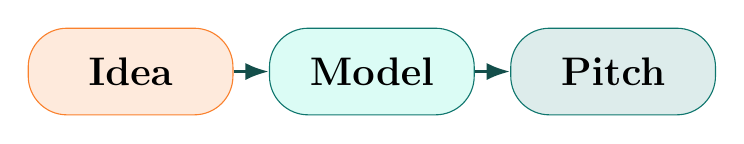
\begin{tikzpicture}[node distance=0.45cm]
\node[rounded corners=14pt, fill=accent3!15, draw=accent3!90, minimum width=2.6cm, minimum height=1.1cm, align=center] (a) {\Large\bfseries Idea};
\node[rounded corners=14pt, fill=accent2!70, draw=accent1, minimum width=2.6cm, minimum height=1.1cm, align=center, right=of a] (b) {\Large\bfseries Model};
\node[rounded corners=14pt, fill=accent1!14, draw=accent1, minimum width=2.6cm, minimum height=1.1cm, align=center, right=of b] (c) {\Large\bfseries Pitch};
\draw[-{Latex[length=3mm,width=2.2mm]}, line width=1.2pt, color=accent4] (a) -- (b);
\draw[-{Latex[length=3mm,width=2.2mm]}, line width=1.2pt, color=accent4] (b) -- (c);
\end{tikzpicture}
\end{center}
\end{frame}

\begin{frame}[plain]
\frametitle{Today's Mission}
\begin{block}{By the end, I will have:}
\begin{itemize}
\large
\item a clear customer
\item a clear problem
\item a CS-connected solution
\item 3 to 5 features or steps
\item a short pitch I can present
\end{itemize}
\end{block}
\vspace{0.2cm}
\begin{center}
\Large\bfseries AI Assistant helps organize and check. You make the business decisions.
\end{center}
\end{frame}

\begin{frame}[plain]
\frametitle{Start With Your Lesson 1 Ticket}
\begin{block}{Find these four things}
\begin{itemize}
\large
\item Business idea
\item Customer or user
\item Problem
\item Computer science connection
\end{itemize}
\end{block}
\vspace{0.2cm}
\begin{center}
\Large If something is missing, use AI Assistant to recover it before building.
\end{center}
\end{frame}

\begin{frame}[plain]
\frametitle{Pitch Deck Structure}
\begin{columns}[T,totalwidth=\textwidth]
\column{0.48\textwidth}
\begin{enumerate}
\large
\item Business name and customer
\item Problem
\item CS-connected solution
\end{enumerate}
\column{0.48\textwidth}
\begin{enumerate}
\large
\setcounter{enumi}{3}
\item Features and how it works
\item Why people would want it
\end{enumerate}
\end{columns}
\vspace{0.25cm}
\begin{center}
\Large\bfseries Keep each slide simple: title, picture or icon, 2 to 3 short bullets.
\end{center}
\end{frame}

\begin{frame}[plain]
\frametitle{Prompt Cards: AI Assistant}
\begin{block}{Click Copy, then paste into AI Assistant}
\begin{itemize}
\large
\item \CopyChip{bmaa1}\hspace{0.5em}\PromptLink{bmaa1}{My business idea is \_\_\_\_. Help me make a 5-slide pitch deck plan.}
\item \CopyChip{bmaa2}\hspace{0.5em}\PromptLink{bmaa2}{My customer is \_\_\_\_ and the problem is \_\_\_\_. Help me explain the problem clearly.}
\item \CopyChip{bmaa3}\hspace{0.5em}\PromptLink{bmaa3}{My solution uses computer science because \_\_\_\_. Help me explain that in Grade 5 words.}
\end{itemize}
\end{block}
\end{frame}

\begin{frame}[plain]
\frametitle{More AI Assistant Prompts}
\begin{block}{Use these when you are building or checking}
\begin{itemize}
\large
\item \CopyChip{bmaa4}\hspace{0.5em}\PromptLink{bmaa4}{Here is my slide draft: \_\_\_\_. What is missing from my business model?}
\item \CopyChip{bmaa5}\hspace{0.5em}\PromptLink{bmaa5}{Help me write a 30-second pitch. Keep it clear and student-friendly.}
\item \CopyChip{bmaa6}\hspace{0.5em}\PromptLink{bmaa6}{Check my business idea for privacy, safety, fairness, and accessibility.}
\end{itemize}
\end{block}
\end{frame}

\begin{frame}[plain]
\frametitle{Worked Example: RecessBuddy}
\begin{block}{Business}
\Large RecessBuddy helps Grade 5 students choose fair teams and games.
\end{block}
\begin{block}{CS solution}
\Large It uses a simple algorithm to balance teams and suggest game choices.
\end{block}
\begin{block}{Feature examples}
\Large Team balancer, game picker, fairness check, class rules reminder.
\end{block}
\end{frame}

\begin{frame}[plain]
\frametitle{Check Before You Present}
\begin{block}{Ask yourself}
\begin{itemize}
\large
\item Did I name the customer?
\item Did I explain the problem?
\item Did I show the CS connection?
\item Did I include safety, privacy, fairness, or accessibility?
\item Can I explain the idea in 30 seconds?
\end{itemize}
\end{block}
\end{frame}

\begin{frame}[plain]
\frametitle{What Not To Do}
\begin{columns}[T,totalwidth=\textwidth]
\column{0.48\textwidth}
\begin{block}{Do}
\begin{itemize}
\large
\item use short bullets
\item check AI suggestions
\item change words so you understand them
\item practice your pitch
\end{itemize}
\end{block}
\column{0.48\textwidth}
\begin{block}{Do Not}
\begin{itemize}
\large
\item paste a full AI essay
\item forget the customer
\item hide the CS connection
\item make promises you cannot support
\end{itemize}
\end{block}
\end{columns}
\end{frame}

\begin{frame}[plain]
\frametitle{Exit Ticket}
\begin{block}{Before you leave, write:}
\begin{itemize}
\large
\item I built \_\_\_\_ today.
\item AI helped me \_\_\_\_.
\item I changed or chose \_\_\_\_ myself.
\item My strongest CS connection is \_\_\_\_.
\item Before I present, I still need to \_\_\_\_.
\end{itemize}
\end{block}
\end{frame}

\end{document}
